
\chapter{A Comparative Analysis of Community Detection Algorithms on Social Networks}



\section{Introduction}
% no \IEEEPARstart

\indent  Networks are used to graphically represent relationship or structure in many complex systems which can be seen in natural, technological or social settings. Understanding the process of formation of such networks or studying why certain systems exhibit a particular structure can provide insights into various phenomena that are commonly seen in real life communities such as diffusion, contagion and influence. These reasons have given birth to the scientific study of networks which became a multi disciplinary field spanning physics, computer science as well as social sciences \cite{aps:1} \cite{aps:2}. One reason for this occurrence is that any system in these fields can be represented in the form of a Network, a second reason is that the theories for studying such Networks have been at the intersection of all these fields \cite{aps:24}. Structurally a network or graph consists of nodes (vertices) and edges. An edge connects typically two nodes but if three or more nodes are connected by a single edge then such an edge is known as a hyperedge and such graphs are called hypergraphs. Other common networks seen in the world are scientific collaboration networks, where the nodes are the researchers and edges between them denote that they are working on the same research topic. An additional example is the Internet which in itself is a massive web graph consisting of web pages (nodes) and hyperlinks (edges). So it is concluded that in general any system can be represented as a network E.g citation networks, social networks, protein communities etc \cite{aps:24}. \\

Most networks of interest demonstrate community structures i.e. nodes (vertices) in them form a dense subgraph. Such subgraphs are referred to as clusters, modules or communities and they exhibit a degree of autonomy in the network\cite{aps:1}. These regions are called autonomous as the nodes in them interact frequently with other nodes in the same clusters than with nodes outside the clusters. Thus, such clusters correspond to entities that interact regularly to perform a function such as hormones responsible for producing an effect in the body or sensors in a home automation system responsible for detecting human presence in a room etc. Real world networks are so large that it is computationally infeasible to develop techniques for their study so in practise, methods are used that can simplify the structure of these large networks before any useful information can be extracted from them. These methods are known as Community Detection algorithms. There are over 100 algorithms that have proliferated in the network literature \cite{aps:10} \cite{aps:8}. The task of identifying communities is important as it offers insight into how a network is organised. This is because individual communities are functional units of the system and they help in understanding the role of the system. \\

The vertices in the network can also be classified on the basis of their roles they play with respect to the communities that they are a part of \cite{aps:24}. A central location makes the nodes important for diffusion of information within the network and so such nodes represent figures of importance with respect to that community. Similarly, the nodes that are located at the boundaries of a community might be acting as brokers for passing information to other communities and possibly play an important role in constraining the dynamics of spreading processes that occur on the network \cite{aps:10}. Other important reasons for creating coarse grain descriptions of networks are that using them missing information can be inferred about nodes by referring to the other nodes in its community or false information can be identified such as presence of an attribute that is uncommon in that community \cite{aps:10} \cite{aps:8}.
\\


Community detection of graphs is however an ill defined problem due to the absence of a universal definition of the object for detection i.e. "community". This has created multiple definitions for Communities, Methods to detect them and Performance evaluation techniques. Due to this ambiguity there is a diffusion of questionable literature in the domain of Network Science. Scientific opinion has changed its perception about networks. In the classical theory, clusters were viewed as dense sub graphs which exhibit a degree of autonomy in the network due to the presence of high edge density between nodes within the cluster than with nodes outside of it. Thus, the classical view relied more on the degree distributions of the nodes in the graph to determine clusters. This created ideas of strong communities and weak communities in a network that depended on the relation between the internal and external degree of the vertices of the graph \cite{aps:27}. The modern view relies more on calculating the probability of edge formation between nodes i.e. the community should be one in which there is a preferential linking pattern. This definition states that nodes in a community would have a higher probability of linking with each other than with nodes of other communities. Another approach that has developed used the link topology of the network and the trajectory of a random walker. The basis of this theory is that a random walk on the network would be concentrated for a longer interval in a dense sub-graph that corresponds to a community. This is because links moving out of a community would be supposedly lesser than those in it \cite{aps:28}. \\

In this paper, an evaluation of eight different state-of-the-art community detection algorithms available in the "igraph" package is performed. The package is a widely used collection of network analysis tools in R, Python, C and C++ and can be used on undirected and directed, weighted and unweighted graphs with overlapping or non overlapping communities. The graphs under examination are "Egonets" or egocentric networks of individuals obtained from Facebook. A review of the most widely used community detection algorithms is given in Section II followed by Experimental work in Section III and Conclusion in Section IV.


\section{Community Detection Algorithms}

\subsection{Walktrap - Computing communities in large networks using random walks}
The algorithm is based on the intuition that random walks on graphs are trapped into a dense part of the graph and such dense sub-graphs corresponds to communities. Walktrap is a agglomerative, hierarchical clustering algorithm that allows finding community structures at different scales. \\

The starting point is an initial partition $P_1$ of the graph with $n$ communities corresponding to the $n$ vertices of the graph i.e.   
Partition $P_1$ = $\lbrace\lbrace v \rbrace, v \epsilon V \rbrace$. A distance measure is used to compute vertex similarity between all adjacent vertices. Then the partition modifies itself by repeating the below operations at each step:\\

\begin{itemize}
\item For two adjacent communities $C_1$ and $C_2$ in $P_k$ merge into single community $C_3$ = $C_1$ $\cup$ $C_2$ and create a new partition $P_{k+1}$ = ($P_k$ : $\lbrace$ $C_1$ , $C_2$ $\rbrace$ ) $\cup \lbrace$ $C_3$ $\rbrace$ if it satisfies a criteria based on the distance between them, and
\item update distance between adjacent communities.\\
\end{itemize}

The algorithm at each step obtains a hierarchical data structure of communities called dendrogram. The algorithm computes the communities in time O(mnH) where n = $\mid V \mid$ vertices, m = $\mid E \mid$ edges and H = height of the dendrogram. For real world graphs which are sparse (m = O( log n)) it comes to O($n^2$ log n) \cite{aps:29}. The tunable parameters in this is the step size of the random walker $t$ which is used to calculate the probability that the random walkers shall move from a vertex $i$ to a vertex $j$. This probability is used to calculate the similarity between vertices and create clusters. The drawback of this method is that it is parameter dependent.\\ 

\subsection{Finding community structure in very large networks}
The "Fastgreedy" technique implemented in the paper has a running time of O($mHlog n$) on a graph with m = $\mid E \mid$ edges, n = $\mid V \mid$ vertices and h = height of the dendrogram \cite{aps:25}. In real world graphs which are sparse the computation time is linear O(n $log^2$ n). The algorithm is based on the greedy optimization of modularity and utilizes shortcuts in the optimization procedure of the original algorithm based on Greedy optimization of modularity \cite{aps:30} and efficient data structures to reduce the time complexity from O($n^2$) on sparse graphs to O(n $log^2$ n). Initially, every vertex belongs to a separate community, and communities are merged iteratively such that each merge is locally optimal. The algorithm stops when the modularity cannot be increased. It has lower time complexity than other techniques and its key drawback is that communities which have nodes and edges below a certain threshold are merged with adjacent communities. The algorithm has detected super communities in graphs that have no underlying clustering structure. It also relies on "modularity optimization" using approximation algorithms to reduce time complexity. However these have produced lower values of modularity than newer versions that have used Simulated Annealing to optimize modularity \cite{aps:33}.\\

\subsection{Finding and evaluating community structure in networks}
The "Edge-betweenness" is a hierarchical decomposition process where edges are removed in the decreasing order of their edge betweenness scores. This is motivated by the fact that edges connecting different communities have a higher probability to occur on the shortest paths between nodes of different communities. However the algorithm has a high running time of O($m^2$n). The repeated calculation of edge betweenness after an edge is removed has to be done for the entire graph. This affects the scalability of the algorithm to large graphs. At each iteration of this approach a full dendrogram is built and a measure to determine the optimal cut of the dendrogram can be made using modularity \cite{aps:31} \cite{aps:32}.  

\subsection{Near linear time algorithm to detect community structures in large-scale networks}
"Label Propagation algorithm" assign an initial unique label at random to the nodes of the network. Each label corresponds to a unique community to which the nodes belongs to. Then a particular node $n_1$ having 'k' neighbours determines it community affiliation based on the most frequent label amongst its neighbours. The problem however is that subgraphs in the
network that are bi-partite or nearly bi-partite in structure lead to oscillations of labels. Hence the label updation step is performed asynchronously. The stopping criteria of the iterative label assigning and re-assigning is till each node has a label to which maximum number of his neighbours belong to. Since the stopping criteria is not a measure to be maximised or minimised the algorithm has no unique solutions in heterogenous graphs with underlying community structure. The method has linear time complexity as every iteration is finished in O($m$) but yields different results based on the initial configuration (which has to be decided randomly), therefore one should run the method a large number of times and then build a consensus labeling, which could be tedious \cite{aps:34}. 

\subsection{Fast unfolding of communities in large networks}
"multilevel.community" is heuristic algorithm for obtaining communities from graphs by optimising the partition measure of modularity \cite{aps:35}. Modularity is the fraction of edges within a community substracted from expected fraction if edges were distributed at random. It is represented by Eqn 1. Since modularity optimization is NP-hard, an approximation algorithm is used that gives a running time of O($nlogn$). 

\begin{equation}
Q = \frac{1}{2m}\sum_{i,j}^{n} [A_{i,j} - \frac{k_i k_j}{2m} ] \delta (C_i C_j) 
\end{equation}

Where,
\begin{itemize}
\item $A_{ij}$ is edge weight between nodes i and j.
\item $k_i$ and $k_j$ are degrees of nodes i and j in case of unweighted graphs.
\item m is the sum of all edge weights in graphs
\item $c_i$ , $c_j$ are communities of nodes.
\item $\delta$ is 1 if edge exists between $c_i$ , $c_j$ and 0 otherwise;
\end{itemize}

The algorithm has two phases that are iteratively repeated:\\
Initially each nodes is assigned to its own unique community. Then for each node, the change in modularity is calculated by removing it from its community and moving it to the community of its neighbours. The change in modularity $\Delta Q$ is given by Eqn 2.

\begin{equation}
\Delta Q = [\frac{\sum_{in}^{}+2K_i,in}{2m} - (\frac{\sum_{tot} + k_i}{2m} )^2] - B
\end{equation}
\begin{equation}
B = [\frac{\sum_{in}^{}}{2m} - (\frac{\sum_{tot}^{}}{2m})^2 - (\frac{k_i}{2m})^2] 
\end{equation}

Where,
\begin{itemize}
\item $\sum_{in}$ is sum of all weights of links inside community to which $i$ is being assigned.
\item $\sum_{tot}$ is sum of all weights of links to nodes in community.
\item $k_i$ is weight degree of $i$
\item $k_i,in$ is the sum of the weights of links between $i$ and other nodes in the cluster.
\item $m$ is the sum of the weights of all links in the network
\end{itemize}

After calculation of $\Delta Q$ for all neighbour nodes of $i$, it is placed in the appropriate community that achieves local optima. This step is repeated for all nodes sequentially till each is assigned to its suitable community. In the second phase, the clusters formed after above step are treated as a single meta-node. The links within a cluster are treated as self loops to the cluster and the links in between clusters are represented as weighted edges between communities. The first pass is repeated again till all communities are organised in a hierarchy. This technique is most suitable for large graphs due to the low time complexity. However, the effects of the technique on the null benchmark i.e. Erdos Renyi random graphs is not verified. The technique is significant for detecting structure in overlapping clusters but not on graphs having non overlapping clusters.

\subsection{Statistical mechanics of community detection}
"spinglass.community" algorithm approaches the problem of community detection as finding the ground state of an infinite ranged Potts spin glass \cite{aps:36}. In this model, each vertex can be in one of $c$ spin states, and the interactions between the particles (i.e. the edges of the graph) specify which pairs of vertices would prefer to stay in the same spin state and which ones prefer to have different spin states. The model is then simulated for a given number of steps, and the spin states of the particles in the end define the communities. The tunable parameter of this technique is the upper limit for the number of clusters $c$ which make it supervised and not suitable for real world graphs. The algorithm is also non deterministic because of simulations needed. In sparse graphs the computational complexity of the algorithm is O($n^{3.2}$)

\subsection{Finding community structure in networks using the eigenvectors of matrices}
"leading.eigenvector.community" algorithm uses the concept of modularity maximization to obtain optimal partitions of the graph \cite{aps:36}. Due to the NP-hard nature of this problem, the modularity matrix is used for calculating the modularity. The eigenvalues and eigenvectors of the matrix are used for clustering. The largest eigenvalue is used to maximise the modularity of the network. This technique belongs to the spectral clustering techniques. This method has higher time complexity than the fast greedy method. Its computational complexity on sparse graphs is O($n^2$).

\subsection{Maps of random walks on complex networks reveal community structure}
"infomap.community" algorithm finds community structure that minimizes the expected description length of a random walker trajectory\cite{aps:36}. The algorithm is based on the Map Equation which yields the description length of an infinite random walk on a graph. The vertices are assigned unique codes and the random walk in the graph is described by the codes of the vertices it visited. Since each vertex has a unique code, the description can be lengthy. The description length can be reduced in a community structure by following the principles of geographic maps where vertices in different communities can have the same code. The best partition is the one that yields minimum description for the random walk.\\

The flow based methods provide different partitions than the methods based on structural features of the network like modularity. The results are striking in graphs having directed edges as these constrain the flow in the graph. The Map equation based techniques give importance to flow and are suitable for networks where structural features affect the dynamics of processes in the network like spread of epidemics, scientific collaborations etc. The runtime of the algorithm is $O(E)$       




% An example of a floating figure using the graphicx package.
% Note that \label must occur AFTER (or within) \caption.
% For figures, \caption should occur after the \includegraphics.
% Note that IEEEtran v1.7 and later has special internal code that
% is designed to preserve the operation of \label within \caption
% even when the captionsoff option is in effect. However, because
% of issues like this, it may be the safest practice to put all your
% \label just after \caption rather than within \caption{}.
%
% Reminder: the "draftcls" or "draftclsnofoot", not "draft", class
% option should be used if it is desired that the figures are to be
% displayed while in draft mode.
%
%\begin{figure}[!t]
%\centering
%\includegraphics[width=2.5in]{myfigure}
% where an .eps filename suffix will be assumed under latex, 
% and a .pdf suffix will be assumed for pdflatex; or what has been declared
% via \DeclareGraphicsExtensions.
%\caption{Simulation results for the network.}
%\label{fig_sim}
%\end{figure}

% Note that the IEEE typically puts floats only at the top, even when this
% results in a large percentage of a column being occupied by floats.


% An example of a double column floating figure using two subfigures.
% (The subfig.sty package must be loaded for this to work.)
% The subfigure \label commands are set within each subfloat command,
% and the \label for the overall figure must come after \caption.
% \hfil is used as a separator to get equal spacing.
% Watch out that the combined width of all the subfigures on a 
% line do not exceed the text width or a line break will occur.
%
%\begin{figure*}[!t]
%\centering
%\subfloat[Case I]{\includegraphics[width=2.5in]{box}%
%\label{fig_first_case}}
%\hfil
%\subfloat[Case II]{\includegraphics[width=2.5in]{box}%
%\label{fig_second_case}}
%\caption{Simulation results for the network.}
%\label{fig_sim}
%\end{figure*}
%
% Note that often IEEE papers with subfigures do not employ subfigure
% captions (using the optional argument to \subfloat[]), but instead will
% reference/describe all of them (a), (b), etc., within the main caption.
% Be aware that for subfig.sty to generate the (a), (b), etc., subfigure
% labels, the optional argument to \subfloat must be present. If a
% subcaption is not desired, just leave its contents blank,
% e.g., \subfloat[].


% An example of a floating table. Note that, for IEEE style tables, the
% \caption command should come BEFORE the table and, given that table
% captions serve much like titles, are usually capitalized except for words
% such as a, an, and, as, at, but, by, for, in, nor, of, on, or, the, to
% and up, which are usually not capitalized unless they are the first or
% last word of the caption. Table text will default to \footnotesize as
% the IEEE normally uses this smaller font for tables.
% The \label must come after \caption as always.
%
%\begin{table}[!t]
%% increase table row spacing, adjust to taste
%\renewcommand{\arraystretch}{1.3}
% if using array.sty, it might be a good idea to tweak the value of
% \extrarowheight as needed to properly center the text within the cells
%\caption{An Example of a Table}
%\label{table_example}
%\centering
%% Some packages, such as MDW tools, offer better commands for making tables
%% than the plain LaTeX2e tabular which is used here.
%\begin{tabular}{|c||c|}
%\hline
%One & Two\\
%\hline
%Three & Four\\
%\hline
%\end{tabular}
%\end{table}


% Note that the IEEE does not put floats in the very first column
% - or typically anywhere on the first page for that matter. Also,
% in-text middle ("here") positioning is typically not used, but it
% is allowed and encouraged for Computer Society conferences (but
% not Computer Society journals). Most IEEE journals/conferences use
% top floats exclusively. 
% Note that, LaTeX2e, unlike IEEE journals/conferences, places
% footnotes above bottom floats. This can be corrected via the
% \fnbelowfloat command of the stfloats package.

\section{Experiments}

The performance of the algorithms in Section II has been evaluated on the dataset provided in Section III (A)

\subsection{Dataset}

The testing of community detection algorithms is done on real or artificially generated networks where ground truth label for the communities is known as in the case of Zachary's karate club dataset or not known as in the case of GN bechmark or the LFR benchmark. The GN benchmark doesn't have the properties of a real network and so the LFR benchmark is used. In the LFR benchmark the vertex degree and community size are power law distributed as is seen in real world communities \cite{aps:26}. In this paper, in the evaluation of the algorithms "Egonets" of 60 user profiles obtained from Facebook are used. Egonets consist of a focal node "ego" and nodes to whom the ego is connected directly called "alters" along with ties between the alters. Such a network has hierarchical, overlapping communities along with homophilous strong ties. 


\begin{table}[!h]
\renewcommand{\arraystretch}{1.3}
\caption{Statistics of the Degree Distribution}
\label{table}
\centering
\begin{tabular}{|c|c|c|c|c|c|}
  \hline
\multicolumn{1}{|c|}{\textbf{Min}} & \multicolumn{1}{c|}{\textbf{I Quad.}} & \multicolumn{1}{c|}{\textbf{Median}} & \multicolumn{1}{c|}{\textbf{Mean}} & \multicolumn{1}{c|}{\textbf{III Quad.}} & \multicolumn{1}{c|}{\textbf{Max}}        \\
  \hline
  0 & 6 & 15 & 24.93 & 33 & 669\\
   \hline
\end{tabular}
\end{table}

\begin{table}[!h]
\renewcommand{\arraystretch}{1.3}
\caption{Statistics of the Order of the Egonets}
\label{table}
\centering
\begin{tabular}{|c|c|c|c|c|c|}
  \hline
\multicolumn{1}{|c|}{\textbf{Min}} & \multicolumn{1}{c|}{\textbf{I Quad.}} & \multicolumn{1}{c|}{\textbf{Median}} & \multicolumn{1}{c|}{\textbf{Mean}} & \multicolumn{1}{c|}{\textbf{III Quad.}} & \multicolumn{1}{c|}{\textbf{Max}}        \\
  \hline
  45 & 116.5 & 219 & 242 & 322 & 670\\
   \hline
\end{tabular}
\end{table}

Table I shows the statistics of the degree distribution obtained from all 60 egonets and Table II shows the summary statistics of number of the nodes of the 60 egonets. Fig 1 shows the histogram of degree distribution which resembles a power law distribution.

\begin{figure}[H]
\centering
\fbox{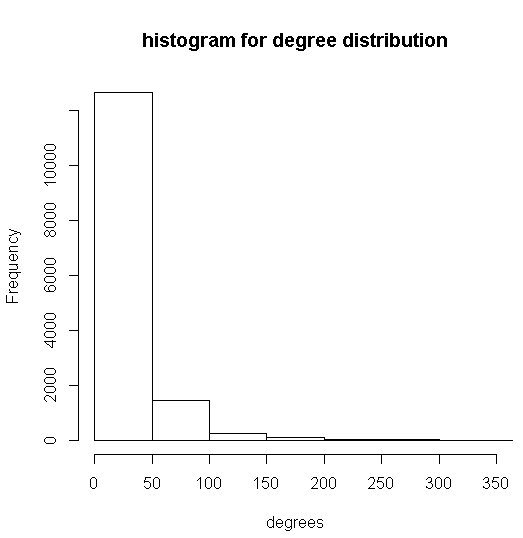
\includegraphics[scale=0.45]{histdeg.png}}
\caption{Histogram of Degree Distribution}
\label{fig 1}
\end{figure}

\subsection{Results}

Table III to X show the performance of the eight algorithms on the datasets. The results represent the modularity metric calculated on the optimal community structure generated on the dataset by the algorithms is given.

\begin{table}[!h]
\renewcommand{\arraystretch}{1.3}
\caption{Statistics of Performance of walktrap.community on Egonets}
\label{table}
\centering
\begin{tabular}{|c|c|c|c|c|c|}
  \hline
\multicolumn{1}{|c|}{\textbf{Min}} & \multicolumn{1}{c|}{\textbf{I Quad.}} & \multicolumn{1}{c|}{\textbf{Median}} & \multicolumn{1}{c|}{\textbf{Mean}} & \multicolumn{1}{c|}{\textbf{III Quad.}} & \multicolumn{1}{c|}{\textbf{Max}}        \\
  \hline
  0.04654 & 0.38017 & 0.50352 & 0.47555 & 0.58518 & 0.84149\\
   \hline
\end{tabular}
\end{table}

\begin{table}[!h]
\renewcommand{\arraystretch}{1.3}
\caption{Statistics of Performance of fastgreedy.community on Egonets}
\label{table}
\centering
\begin{tabular}{|c|c|c|c|c|c|}
  \hline
\multicolumn{1}{|c|}{\textbf{Min}} & \multicolumn{1}{c|}{\textbf{I Quad.}} & \multicolumn{1}{c|}{\textbf{Median}} & \multicolumn{1}{c|}{\textbf{Mean}} & \multicolumn{1}{c|}{\textbf{III Quad.}} & \multicolumn{1}{c|}{\textbf{Max}}        \\
  \hline
  0.2411 & 0.4220 & 0.4927 & 0.4960 & 0.5813 & 0.8299\\
   \hline
\end{tabular}
\end{table}

\begin{table}[!h]
\renewcommand{\arraystretch}{1.3}
\caption{Statistics of Performance of edge.betweeness.community on Egonets}
\label{table}
\centering
\begin{tabular}{|c|c|c|c|c|c|}
  \hline
\multicolumn{1}{|c|}{\textbf{Min}} & \multicolumn{1}{c|}{\textbf{I Quad.}} & \multicolumn{1}{c|}{\textbf{Median}} & \multicolumn{1}{c|}{\textbf{Mean}} & \multicolumn{1}{c|}{\textbf{III Quad.}} & \multicolumn{1}{c|}{\textbf{Max}}        \\
  \hline
  0.1566 & 0.3600 & 0.4896 & 0.4719 & 0.5921 & 0.8528\\
   \hline
\end{tabular}
\end{table}

\begin{table}[!h]
\renewcommand{\arraystretch}{1.3}
\caption{Statistics of Performance of label.propagation.community on Egonets}
\label{table}
\centering
\begin{tabular}{|c|c|c|c|c|c|}
  \hline
\multicolumn{1}{|c|}{\textbf{Min}} & \multicolumn{1}{c|}{\textbf{I Quad.}} & \multicolumn{1}{c|}{\textbf{Median}} & \multicolumn{1}{c|}{\textbf{Mean}} & \multicolumn{1}{c|}{\textbf{III Quad.}} & \multicolumn{1}{c|}{\textbf{Max}}        \\
  \hline
  0.0000 & 0.3323 & 0.4824 & 0.4469 & 0.5820 & 0.8482\\
   \hline
\end{tabular}
\end{table}

\begin{table}[!h]
\renewcommand{\arraystretch}{1.3}
\caption{Statistics of Performance of multilevel.community on Egonets}
\label{table}
\centering
\begin{tabular}{|c|c|c|c|c|c|}
  \hline
\multicolumn{1}{|c|}{\textbf{Min}} & \multicolumn{1}{c|}{\textbf{I Quad.}} & \multicolumn{1}{c|}{\textbf{Median}} & \multicolumn{1}{c|}{\textbf{Mean}} & \multicolumn{1}{c|}{\textbf{III Quad.}} & \multicolumn{1}{c|}{\textbf{Max}}        \\
  \hline
  0.2523 & 0.4546 & 0.5264 & 0.5205 & 0.6141 & 0.8557\\
   \hline
\end{tabular}
\end{table}

\begin{table}[!h]
\renewcommand{\arraystretch}{1.3}
\caption{Statistics of Performance of spinglass.community on Egonets}
\label{table}
\centering
\begin{tabular}{|c|c|c|c|c|c|}
  \hline
\multicolumn{1}{|c|}{\textbf{Min}} & \multicolumn{1}{c|}{\textbf{I Quad.}} & \multicolumn{1}{c|}{\textbf{Median}} & \multicolumn{1}{c|}{\textbf{Mean}} & \multicolumn{1}{c|}{\textbf{III Quad.}} & \multicolumn{1}{c|}{\textbf{Max}}        \\
  \hline
  0.2573 & 0.4379 & 0.4988 & 0.4908 & 0.5640 & 0.7188\\
   \hline
\end{tabular}
\end{table}

\begin{table}[!h]
\renewcommand{\arraystretch}{1.3}
\caption{Statistics of Performance of leading.eigenvector.community on Egonets}
\label{table}
\centering
\begin{tabular}{|c|c|c|c|c|c|}
  \hline
\multicolumn{1}{|c|}{\textbf{Min}} & \multicolumn{1}{c|}{\textbf{I Quad.}} & \multicolumn{1}{c|}{\textbf{Median}} & \multicolumn{1}{c|}{\textbf{Mean}} & \multicolumn{1}{c|}{\textbf{III Quad.}} & \multicolumn{1}{c|}{\textbf{Max}}        \\
  \hline
  0.2372 & 0.4250 & 0.5039 & 0.5050 & 0.6013 & 0.8321\\
   \hline
\end{tabular}
\end{table}

\begin{table}[H]
\renewcommand{\arraystretch}{1.3}
\caption{Statistics of Performance of infomap.community on Egonets}
\label{table}
\centering
\begin{tabular}{|c|c|c|c|c|c|}
  \hline
\multicolumn{1}{|c|}{\textbf{Min}} & \multicolumn{1}{c|}{\textbf{I Quad.}} & \multicolumn{1}{c|}{\textbf{Median}} & \multicolumn{1}{c|}{\textbf{Mean}} & \multicolumn{1}{c|}{\textbf{III Quad.}} & \multicolumn{1}{c|}{\textbf{Max}}        \\
  \hline
  0.04513 & 0.41261 & 0.50660 & 0.48933 & 0.60126 & 0.84931\\
   \hline
\end{tabular}
\end{table}

The highest mean modularity is obtained by the multilevel community detection algorithm. The real world datasets exhibit a community structure which might not be based on modularity. A second evaluation metric is used to calculate the edit distance between the ground truth communities in the dataset and the predicted communities by the algorithms.

\begin{table}[!h]
\renewcommand{\arraystretch}{1.3}
\caption{Running time of Algorithms on Egonets}
\label{table}
\centering
\begin{tabular}{|c|c|c|c|c|c|c|}
  \hline
\multicolumn{1}{|c|}{\textbf{Name}} & \multicolumn{1}{|c|}{\textbf{Min}} & \multicolumn{1}{c|}{\textbf{I Quad.}} & \multicolumn{1}{c|}{\textbf{Median}} & \multicolumn{1}{c|}{\textbf{Mean}} & \multicolumn{1}{c|}{\textbf{III Quad.}} & \multicolumn{1}{c|}{\textbf{Max}}        \\
  \hline
  EDG & 2583 & 4231 & 4641 & 5711 & 5519 & 11111\\
  \hline
  IMaP & 0.01 & 0.05 & 0.115 & 0.247 & 0.360 & 1.530\\
  \hline
  MLTL & 0.01 & 0.01 & 0.01 & 0.012 & 0.02 & 0.05\\
  \hline
  WLK & 0.00 & 0.01 & 0.02 & 0.046 & 0.052 & 0.47\\
  \hline
  FTG & 0.00 & 0.00 & 0.02 & 0.08 & 0.082 & 1.12\\
  \hline
  LDG & 0.00 & 0.04 & 0.09 & 0.14 & 0.152 & 1.96\\
  \hline
  LBP & 0.00 & 0.00 & 0.00 & 0.0048 & 0.01 & 0.02\\
  \hline
  SPG & 2.17 & 7.01 & 16.7 & 31.2 & 36.04 & 250.45\\
  
   \hline
\end{tabular}
\end{table}

Table XI shows the running time in millisecs needed by the algorithms on the dataset. The average nodes in the network were 242 with the minimum size of 45 and maximum of 670. The label propagation algorithm has obtained the lowest running time on the datasets. The highest time complexity is seen in the edge betweenness algorithm and it proves that it may not scale well to large datasets.

\subsection{Edit Distance metric}

Edit distance calculates the minimum number of edit operations needed for transformation of the predicted solution with the actual solution. Each of the following operations cost one edit: 
\begin{itemize}
\item Add user to an existing circle.
\item Remove user from a circle.
\item create a circle with one user.
\item delete a circle with one user.
\end{itemize}

\begin{table}[H]
\renewcommand{\arraystretch}{1.3}
\caption{Edit Distance of Algorithms on Egonets}
\label{table}
\centering
\begin{tabular}{|c|c|c|}
  \hline
\multicolumn{1}{|c|}{\textbf{Sr No.}} & \multicolumn{1}{|c|}{\textbf{Name}} & \multicolumn{1}{c|}{\textbf{Edit Distance}}  \\
  \hline
  1 & edge.betweenness & 14284\\
   \hline
  2 & multilevel & 15162\\
   \hline
  3 & infomap & 13988\\
   \hline
  4 & label.propagation & 14538\\
   \hline
  5 & spinglass & 15256\\
   \hline
  6 & fastgreedy & 14736\\
   \hline
  7 & walktrap & 14696\\
   \hline
  8 & leading.eigenvector & 15304\\
   \hline
\end{tabular}
\end{table}

From comparison of the edit distance metric shown in Table XII the infomap algorithm has obtained the lowest edit cost amongst the algorithms.



\section{Conclusion}
Egocentric networks present a challenge for community detection as the community structure in them is defined by the 'ego' to which the network belongs to. The presence of ground truth labels to the communities allows one to evaluate the precision of the algorithms effectively. The choice of algorithms therefore can be based on objective criteria like accuracy, running time and computational complexity. From our results, all algorithms with the exception of spinglass and edge betweenness were scalable and could be used on large networks. The partition quality is also an indicator of the accuracy of the algorithm, however real world datasets might not be based on optimum modularity. On this scale, the algorithms had mean modularity was close to each other. This was seen even in the case of algorithms like infomap and label propagation that don't partition based on optimum modularity. Finally, real world datasets exhibit heterogeneity due to which they may contain noise and also they do not have an fixed objective criteria for creation of communities. Therefore the edit distance measure showed high cost which meant that the partitions created by the algorithms had disagreements with the partitions made by the respective users or 'egos'.    
